Even though the robot chosen is a collaborative robot, the payload is a metal sheet which poses a safety concern for the human operator.
To avoid such scenarios a safety fence is installed at the boundary of robotic workcell as mentioned in section \ref{sub:safety-fence}.
Still several considerations are required for the safe operation of robot in the workcell like the speed at which the robot should operate. These factors depends on the payload attached to the robot and the distance between payload and the joint axis 1 or joint axis 2.
Following subsections explains the reasoning behind safety parameters that were considered for the safe operation of \hyperref[acro:KR]{KR1410}.

\subsection{Payload}
\label{subsec:payload}
The pneumatic parallel gripper, manual quick-change system and robotic camera constitutes a weight of 2.0 \textit{kg}.
This is the fixed load on the tool flange center (\hyperref[acro:TFC]{TFC}). The sheet metal parts count as the payload.
It is a variable load of only 0.1 \textit{kg} and is thus ignored for the calculations in \ref{subsec:stoppage-distance}.


\begin{figure}[h]
    \centering
    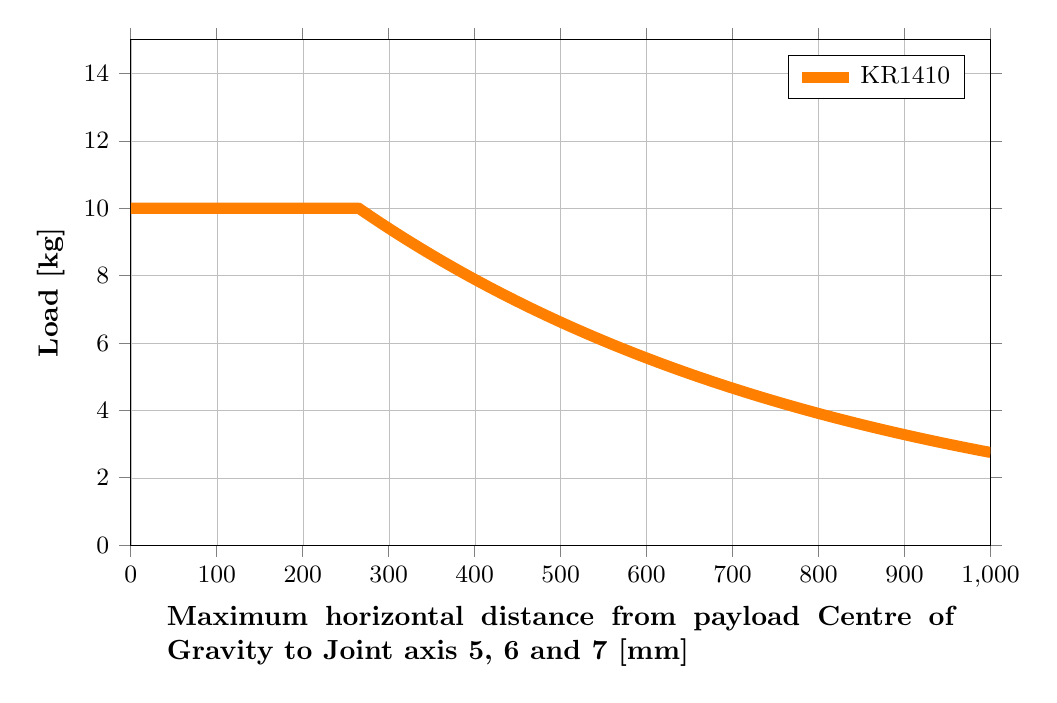
\begin{tikzpicture}
        \begin{axis}[
            width=12.5cm,
            height=8cm,
            grid=both,
            grid style={line width=.1pt, draw=gray!30},
            major grid style={line width=.1pt,draw=gray!50},
            xlabel={\parbox{10cm}{Maximum horizontal distance from payload Centre of Gravity to Joint axis 5, 6 and 7 [mm]}},
            ylabel={\textbf{Load [kg]}},
            xmin=0, xmax=1000,
            ymin=0, ymax=15,
            legend pos=north east,
            legend style={font=\small},
            ylabel near ticks,
            xlabel near ticks,
            tick align=outside,
            tick label style={font=\small},
            label style={font=\bfseries},
        ]
    
        % KR1410 (orange)
        \addplot [
            color=orange,
            line width=4pt,
            % ultra thick,
            domain=0:1000,
            samples=1000,
        ]
        {x <= 265 ? 10 : 10*exp(-0.001756*(x-265))};
        \addlegendentry{KR1410}
        \end{axis}
    \end{tikzpicture}
    
    \caption{Payload diagram for KR1410 manipulator}
    \label{fig:kr1410-payload-diagram}
\end{figure}


The permissible payload is constrained due to the static torque limit of the wrist joints. The payload is
reduced according to the proximity of the payload's center of gravity in relation to joint axis 5, 6 and 7. \cite[page 35]{kassow-manual}
Only about 1100 \textit{mm} out of 1400 \textit{mm} of workspace is utilized by the \hyperref[acro:KR]{KR} in the workcell. 
Figure \ref{fig:kr1410-payload-diagram}
illustrates the allowable payload as a function of distance. It's evident from this it is safe to operate with a load a 2.0 \textit{kg}.

\subsection{Stopping Distance}
\label{subsec:stoppage-distance}
The stopping time \hyperref[sym:t-brake]{$t_{\text{brake}}$} and distance \hyperref[sym:s-brake]{$s_{\text{brake}}$} should be kept as low as possible. \hyperref[sym:s-brake]{$s_{\text{brake}}$} is set at 60 \textit{mm} and \hyperref[sym:t-brake]{$t_{\text{brake}}$} at 0.2 \textit{s} for safety reason.
According to \cite[page 35]{kassow-manual}, the time and distance it takes to stop the robot, for instance with an emergency stop or protective stop, depends on the load, speed
and configuration of the robot. Conservative estimations of \hyperref[sym:t-brake]{$t_{\text{brake}}$} and \hyperref[sym:s-brake]{$s_{\text{brake}}$} are made by firstly identifying how fast the
slowest joints can decelerate. This depends on the payload, the direction in which the payload is heading
relative to gravity, and the distance between the load or \hyperref[acro:TFC]{TFC} and joint axis 1 or 2, depending on whatever
distance is the longest.
The values can be seen in the Table \ref{tab:braking_accelerations}.


    \begin{table}[h]
        \centering
        \renewcommand{\arraystretch}{1.2} % Adjusts row height
        \small
        \setlength{\tabcolsep}{4.5pt} % Adjusts column spacing
        \begin{tabular}{cc|*{7}{c}}
            \hline
            \textbf{Load} & \textbf{Direction} & 
            \multicolumn{7}{c}{\textbf{Distance from Joint axis 1 or 2 to Load center}} \\
            \textbf{[kg]} & \textbf{[deg]} & 
            \multicolumn{7}{c}{\textbf{of gravity or TFC, whichever is larger}} \\
            \cline{3-9}
            & & 800-950 & 700-800 & 600-700 & 500-600 & 400-500 & 300-400 & 0-300 \\
            \hline
            \multirow{4}{*}{0-4}  & 0-40  & 895  & 1026 & 1304 & 1663 & 2131 & 2724 & 3437 \\
                                & 40-80 & 1433 & 1578 & 1745 & 2132 & 2522 & 3131 & 3724 \\
                                & 80-120 & 1378 & 1549 & 1720 & 2115 & 2643 & 3165 & 4045 \\
                                & 120-160 & 1861 & 2040 & 2371 & 2773 & 3259 & 3824 & 4342 \\
            \hline
        \end{tabular}
        \caption{Braking accelerations \hyperref[sym:a-brake]{$a_{\text{brake}}$} \textit{$[\text{deg/s}^2]$} for KR1410}
        \label{tab:braking_accelerations}
    \end{table}

    The stopping time \hyperref[sym:t-brake]{$t_{\text{brake}}$} and stopping distance \hyperref[sym:s-brake]{$s_{\text{brake}}$} can now be conservatively estimated based on the knowledge of the set speed
    in the robot program and equations \ref{eq:t-brake} and \ref{eq:s-brake}. Joint speed \hyperref[sym:omega]{$\omega$} is used for \hyperref[acro:Move J]{Move J} and linear speed \hyperref[sym:v-max]{$v_{\text{max}}$} for \hyperref[acro:Move L]{Move L} and \hyperref[acro:Move S]{Move S} commands.
    By default, in normal run mode of program, \hyperref[acro:Move J]{Move J} command runs a maximum joint speed of 90 \textit{deg/s} and
    \hyperref[acro:Move L]{Move L} command runs a maximum linear speed of 1000 \textit{mm/s}. This linear speed can be converted to joint speed
    using the equation \ref{eq:omega}.

    \begin{equation}
        \omega = \frac{180 \, v_{\text{max}}}{r\pi} \quad [\text{deg} \, s^{-1}]
        \label{eq:omega}
    \end{equation}
                
    \begin{equation}
        t_{\text{brake}} = \frac{\omega}{a_{\text{brake}}} + 0.020 \quad [\text{s}]
        \label{eq:t-brake}
    \end{equation}
        
    \begin{equation}
        s_{\text{brake}} = \left(\frac{t_{\text{brake}} + 0.02}{360}\right) \pi r w \quad [\text{mm}]
        \label{eq:s-brake}
    \end{equation}

    From these equations, it is evident that \hyperref[sym:t-brake]{$t_{\text{brake}}$} and \hyperref[sym:s-brake]{$s_{\text{brake}}$} are directly proportional to \hyperref[sym:omega]{$\omega$}.
    To avoid triggering joint torque value exceeded error and for safe operation of robot, the joint speed \hyperref[sym:omega]{$\omega$} is reduced for specifically difficult trajectory execution or when the distance
    between joint axis 1 or joint axis 2 and \hyperref[acro:TFC]{TFC} is large. For example, to keep the same \hyperref[sym:t-brake]{$t_{\text{brake}}$} for a distance of 900 \textit{mm} between Joint axis 1 and payload
    but two robot configuration of 0-40 \textit{deg} and 120-160 \textit{deg}, joint speed \hyperref[sym:omega]{$\omega$} must be halved
    for 0-40 \textit{deg} robot configuration.

\subsection{Safety zones}
\label{subsec:safety-zones}

Safety Zones represent virtual boundaries in the robot workspace. The robot will reduce its speed or stop
completely if any part of the robot enters the safety zone. This can be used for protection of sensitive
equipment or areas with human presence. \cite[page 96]{kassow-software-manual}


\begin{figure}[h]
    \centering
    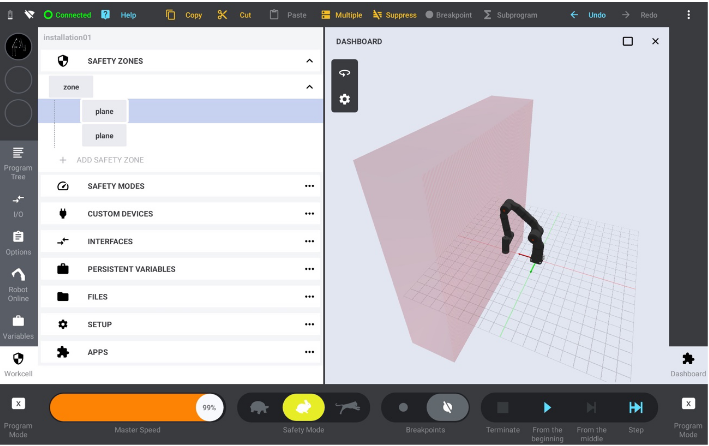
\includegraphics[width=0.7\textwidth]{figures/safety-zones.png}
    \caption{Addition of safety zones to the robotic workcell}
    \label{fig:safety-zones}
\end{figure}

A safety zone for unloading station, storage station, bending machine and terminal operating
robot is created. Since the
robot can actually touch the floor, an additional safety zone is added for the floor. 
The robot will stop immediately if it ever exceeds the safety zone boundary. If it exceeds, 
then the operator
has to manually move the robotic arm back inside the safety zone. 

\subsection{Safety functions}
\label{subsec:safety-functions}
Safety functions evaluate external and internal signals of the whole system which can act immediately to
halt the robot or cut him loose from power if necessary. 
The safety function of \hyperref[acro:KR]{KR1410} complies with EN ISO 13849-1:2015. \cite{ISO13849}
\cite[page 13]{kassow-software-manual}

\begin{figure}[h]
    \centering
    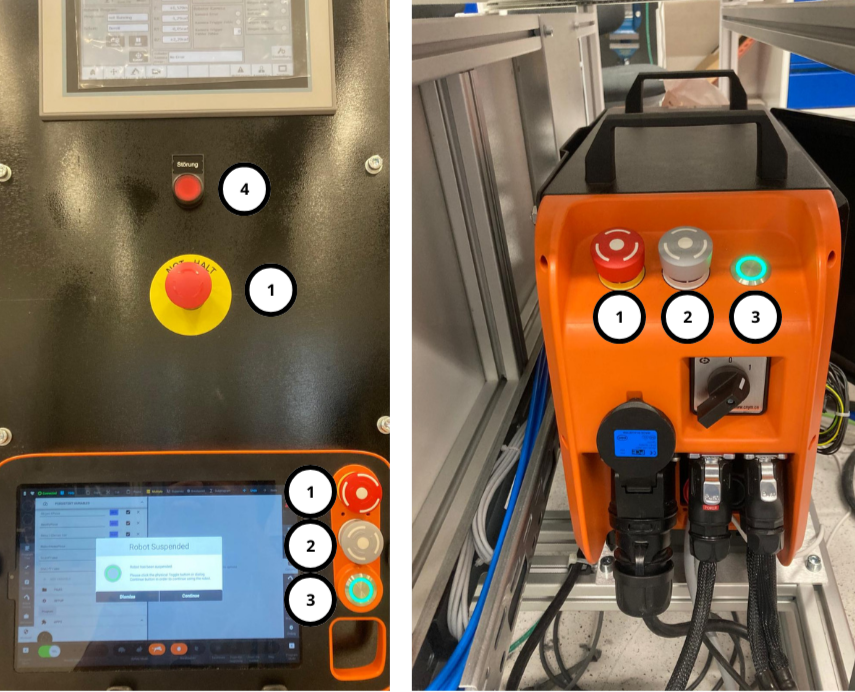
\includegraphics[width=0.7\textwidth]{figures/safety-buttons.png}
    \caption{Safety buttons. 1) Emergency STOP 2) Protective STOP 3) Robot State 4) Reset \hyperref[acro:PLC]{PLC} fault}
    \label{fig:safety-buttons}
\end{figure}

In the main program of teach pendant, there are two sequences programmed to run in parallel to halt or stop the program if a signal is detected
from the \hyperref[acro:PLC]{PLC}. The former sequence pauses the robot motion and waits for a new signal from \hyperref[acro:PLC]{PLC} to continue the robot motion from the same configuration while the latter sequence triggers the E-Stop on the robot and stops the robot immediately. 



\subsubsection{Protective STOP}
The Protective STOP can be used interactively by the operator to pause and continue the running program.
After the protective STOP is released, the program can continue running its normal operation.

\subsubsection{Emergency STOP}
The emergency STOP buttons of robot are present at both teach pendant and robot controller. These buttons are used to engage inbuilt safety measures and halt the robot in order to
prevent a potentially hazardous situation
The emergency STOP always provoke immediate halt of the robot, followed by the power cut to all
executive parts of the robot.

Besides these E-stop buttons, there are three more E-Stop in the workcell. Two are placed on the bending machine and one on the front panel of unloading station as shown in figure \ref{fig:safety-buttons}. The emergency stop buttons not only stops the robot but also the bending machine and unloading station mechatronic system.


\vspace{1\baselineskip}
